
\section{Derivable functions can be described in first-order logic}
\label{sec:to-logic}
The goal of this section is to show the right-to-left implication of Theorem~\ref{thm:main}, which says that derivable functions can be implemented by first-order transductions. 

As discussed in the body of the paper, we proceed by induction on the derivation. During this induction, we will need to show that every prime function is a first-order transduction. Prime functions are not tree-to-tree functions, instead they transform dataypes into datatypes. This is the reason why we need 
\begin{itemize}
\item to generalize tree-to-tree transductions into  transductions that can transform models over arbitrary vocabularies (and not only the vocabulary of trees). 
\item show how datatypes (terms, pairs, copairs and folds) can be encoded as models over a well chosen vocabulary. More precisely, we will associate to every datatype $\rSigma$ a relational vocabulary that we call \emph{vocabulary of $\rSigma$}. Then we will define the function
\begin{align*}
\underline{\bullet}: \rSigma \xrightarrow{\qquad} \text{Vocabulary of $\rSigma$}
\end{align*} 
which encodes the inhabitants of $\rSigma$ as models over the vocabulary of $\rSigma$.
\end{itemize}
 
 Right-to-left implication can be then generalized to the following statement, more suited to a proof by induction

\begin{proposition}\label{prop:main-right-to-left}
Let $\rGamma$ and $\rSigma$ be two datatype.  For every derivable function $\ranked{f}$, there is a first-order transduction $g$ such that the following diagram commutes
  \begin{align*}
  \xymatrix@C=2.8cm{
          \rSigma 
        \ar[d]_{\substack{\underline{\bullet}}}
        \ar[r]^-{\ranked{f}}
        &
    \rGamma \ar[d]^{\substack{\underline{\bullet}}}
        \\
      \text{Vocabulary of $\rSigma$}
        \ar[r]_-{g}
        &
    \text{Vocabulary of $\rGamma$}   
    } 
\end{align*}  
\end{proposition}

The rest of this section is organized as follows. We define first-order transductions transforming arbitrary models in Section~\ref{sec:fo-transduction-def}. In Section~\ref{sec:data-as-models} we define the vocabulary of a datatype and show the encoding $\underline{\bullet}$ of data into models. Finally, we prove Proposition~\ref{prop:main-right-to-left} which gives as a corollary the right-to-left implication of Theorem~\ref{thm:main}.

\subsection{First-order transductions}\label{sec:fo-transduction-def}
The following definition introduces first-order transductions, which generalizes tree-to-tree transductions given in Definition~\ref{def:fo-transduction}.  

\begin{definition}[First-order transduction]\label{def:fo-transduction-gen}\ 
\begin{enumerate}
    \item \emph{Copying.} Fix some  relational vocabulary $\ranked \sigma$ and let $k \in \set{1,2,\ldots}$. Define $k$-copying to be the operation 
    $$\begin{array}{lll}
     \text{models over $\ranked \sigma$} & \to & 
     \begin{array}{c}
     \text{models over $\ranked \sigma$}\\ 
     \text{extended with a $k$-ary relation $\mathrm{copy}$}
     \end{array}
    \end{array}$$
which inputs a model $\mathbb A$, and outputs $k$ disjoint copies of $\mathbb A$, where the  $\mathrm{copy}$ relation is interpreted as the set of tuples $(a_1,\ldots,a_k)$ such that, for  some $a \in \mathbb A$, the first copy of $a$ is  $a_1$, the second copy of $a$ is $a_2$, etc. The $\mathrm{copy}$ relation  is not commutative, because we distinguish the copies.
\item    \emph{Non-copying first-order transduction.} The syntax of a \emph{non-copying first-order transduction}  is given by:
\begin{enumerate}
    \item Input relational vocabulary $\ranked\sigma$ and output relational vocalbulary $\ranked{\gamma}$.
    \item A first-order \emph{universe formula} $\varphi(x)$ over $\ranked{\sigma}$.
    \item For every relation $R$ in vacubulary $\ranked{\gamma}$, a first-order  formula $\varphi_R(x_1,\ldots,x_{\arity R})$ over $\ranked{\sigma}$.
\end{enumerate}
The semantics of a non-copying first-order transduction is  a function
\begin{align*}
    \text{models over $\ranked\sigma$} \quad \to \quad \text{models over $\ranked\gamma$}
\end{align*}
defined as follows. If the input model is $\mathbb A$, then the output model is defined as follows: the universe is elements of $\mathbb A$ which satisfy the universe formula, and each relation $R$ is interpreted as those tuples that satisfy $\varphi_R$. 
\item \emph{First-order transductions.} A \emph{first-order transduction} is defined to be any  composition of $k$-copying (for some $k$) followed by a non-copying first-order transduction. 
 \end{enumerate}
\end{definition}

When restricted to the vocabulary of trees, Definition~\ref{def:fo-transduction-gen} of first-order transductions does not match exactly the definition of tree-to-tree transductions given in the body of the paper. More precisely, the $k$-copying operation is not exactly the same in these two definitions. They are however equivalent in the sens that, when restricted to the vocabulary of trees, we can find for every first-order transduction in the sens of definition~\ref{def:fo-transduction-gen}, a tree-to-tree transduction as in Definition~\ref{def:fo-transduction}, and conversely.
 
\subsection{Data as models.}\label{sec:data-as-models}
Let us show how to encode datatypes as relational vocabularies and data as models over these vocabularies. 
\begin{definition}[Associated models for terms, pairs, co-pairs and tensors.] \label{def:type-model} To each type  $\rSigma$ we associate a vocabulary, called the \emph{vocabulary of $\rSigma$}, and a map 
    \begin{align*}
        a \in \rSigma \qquad \mapsto \qquad \underbrace{\underline a \in \text{models over the  vocabulary of  $\rSigma$}}_{\text{associated model of $a$}}.
    \end{align*}
    Furthermore, for each $a \in \rSigma$ we  distinguish a  sequence (whose length is the arity of $a$) of elements in $\underline a$, which are called the ports of $\underline a$.   The definitions are by induction on the structure of $\rSigma$, as given below.
    \begin{itemize}
        \item \emph{Finite ranked sets.} Elements of a ranked set   \begin{align*}
        \rSigma =  \set{a_1,\ldots,a_k}
        \end{align*} are modeled  using a vocabulary which has unary relations $a_1,\ldots,a_k$ and $P_1,\ldots,P_m$ where $m$ is the maximal arity of elements in $\rSigma$. 
        For $a \in \rSigma$ of arity $n$, the  universe of $\underline a$ is $\set{0,1,\ldots,n}$, with the ports being $1,\ldots,n$. 
            The  relation $P_i$  is interpreted as $\set i$ when $i \in \set{1,\ldots,n}$ and as the empty set otherwise. The relation $a_i$ is interpreted as $\set 0$ when $a = a_i$ and as the empty set otherwise. 
        \item \emph{Coproduct.}  Elements of the coproduct $\ranked{\Sigma_1 + \Sigma_2}$ are modeled using the disjoint union of the vocabularies of $\ranked{\Sigma_1}$ and $\ranked{\Sigma_2}$. 
            If an element of the coproduct comes from $\ranked{\Sigma_1}$, then its associated model is defined as for the type $\ranked{\Sigma_1}$, with  the remaining relations from the vocabulary of   $\ranked{\Sigma_2}$ interpreted   as empty sets. The definition is analogous for  elements from $\ranked{\Sigma_2}$. 
        \item \emph{Tensor product.}   Tensor pairs in   $\ranked{\Sigma_1 \product \Sigma_2}$ are modeled
        using the disjoint union of the vocabularies of $\ranked{\Sigma_1}$ and $\ranked{\Sigma_2}$. 
            For  $\tensorpair{a_1,a_2}$, the associated model is    the disjoint union $\underline{a_1} + \underline {a_2}$, with the relations of $\underline {a_1}$ using the  vocabulary of ${\ranked{\Sigma_1}}$, and the relations of $\underline {a_2}$ using the vocabulary  ${\ranked{\Sigma_1}}$. 
            If $n_1$ is the arity of $a_1$, then the first $n_1$ ports are inherited from  $\underline {a_1}$ and the remaining ports are inherited from  $\underline {a_2}$.
        \item \emph{Cartesian product.}   Cartesian pairs in  $\ranked{\Sigma_1 \product \Sigma_2}$ are modeled  using the disjoint union of the vocabularies of $\ranked{\Sigma_1}$ and $\ranked{\Sigma_2}$, plus an extra binary relation $R$.  
            The model associated to a Cartesian pair   $ (a_1,a_2)$,  is      the disjoint union $\underline{a_1} +  \underline {a_2}$, in the same sense as in the previous item for $\product$,  with the binary relation $R$ interpreted as 
                \begin{align*}
                   \quad \set{(\text{$i$-th port of $\underline {a_1}$}, \text{$i$-th port of $\underline a_2$}): i \in [1,\text{arity of $(a_1,a_2)$}]} 
                \end{align*}
                The ports are inherited from   $\underline {a_1}$.
        \item \emph{Folding.}   For $k \in \set{1,2,\ldots}$, elements of   $\reduce k \rSigma$ are modeled using the  vocabulary of $\rSigma$ plus two extra binary relations $\portord$ and $R$. If $a \in \rSigma$ has arity $nk$, then the model associated to $a/f$ -- which has arity $n$ --   is obtained from  $\underline{a}$ by adding a copy of the model below, where $\sqsubset$ is the natural ordering on integers
                \begin{align*}
                (\set{1,\ldots,n}, \portord),
                \end{align*}
whose elements are used as the ports, and interpreting the binary relation $R$ as
        \begin{align*}
        \set{(\text{$i$-th port of $\underline a$},f(i)) : i \in \set{1,\ldots,nk}}
        \end{align*}
                
                
        \item \emph{Terms.}   Terms in $\tmonad \rSigma$ are modeled using vocabulary of $\rSigma$ extended with two fresh binary relations $\anceord$ and $\portord$. 
          Let $t \in \tmonad \rSigma$. Consider the disjoint union of models
            \begin{align}\label{eq:non-port}
                 \coprod_{x \in \text{non-port nodes in $t$}} \underline{a(x)},
            \end{align}
         where  $\underline a(x)$ is the model over vocabulary of $\rSigma$ that  is defined by induction assumption.   In the above  disjoint union, the same vocabulary, namely the vocabulary of $\rSigma$,  is used  for all parts of the disjoint union. Next, consider  the model
            \begin{align}\label{eq:ports}
            (\set{1,\ldots,n}, \portord)
            \end{align}
            where $\portord$ is the natural ordering on $\set{1,\ldots,n}$. 
            The model of $t$ is defined by taking the disjoint union of the models in~\eqref{eq:non-port} and~\eqref{eq:ports}, and defining the descendent relation $\anceord$ as the set of pairs $(u,v)$ such that:
            \begin{itemize}
            \item either $u$ is the $i$-th port of $\underline{a(x)}$ for some node $x$ of $a$, $v$ is a port of $\underline{a(y)}$ for some node $y$ which is a descendent of the $i$-th child of $x$.
            \item or $u$ is the $i$-th port of $\underline{a(x)}$ for some node $x$ of $a$, $v=j\in\{1,\dots,n\}$ and the $j$-th port of $a$ is a descendent of the $i$-th child of $x$.
            \end{itemize} 

            % It  consists of all pairs $(u,v)$ such that $u$ is the $i$-th port of $\underline{a(x)}$  some non-port node $x$, and $v$ belongs to $\underline{a(y)}$ for some node (possibly a port) $y$ which is a descendant (not necessarily proper) of the $i$-th child of $x$. The binary relation $\portletter$ is the total order 
           % The ports are taken from the structure~\eqref{eq:ports}.
    \end{itemize}
\end{definition}

The above  definition creates a certain ambiguity for trees, because if $t$ is a tree over a finite ranked set $\rSigma$, then $\underline t$ can be understood in two ways: as per  Definition~\ref{def:tree-model} for trees, or as per Definition~\ref{def:type-model} when $t$ is viewed as a special case of a term $t \in \tmonad \rSigma$. Since we only use first-order transductions to transform relational structures,  this ambiguity is not a problem, because one can easily define first-order transductions which map one definition of $\underline t$ to the other.


\subsection{Proof of Proposition~\ref{prop:main-right-to-left}}
The proof proceeds by induction, following the definition of derivable functions. All the cases are easy, and consist mainly on unfolding the definitions. We will treat only the case of the prime function $\unit$  to illustrate this process.
    
    In the following, it will be convenient to use, as part of the vocabulary of $\rSigma$, the unary relation  $\mathsf{Port}_\rSigma$ which selects the ports of the structures over the vocabulary of $\rSigma$; and the binary relation $\sqsubset_\rSigma$ which orders these ports. By induction on $\rSigma$, we can show that both relations are definable by first-order formulas over  the vocabulary of $\rSigma$.
    
    
   Given an element $x$ of $\rSigma$, let us show how  $\unit(x)$ can be implemented using a FO transduction.  The copying constant is 2,
    the first copy will contain the whole structure $\underline{x}$ and the second copy will select only the ports of $\underline{x}$ which will serve as the ports of the structure $\underline{\unit(x)}$, as illustrated by the following picture 
\begin{center}
    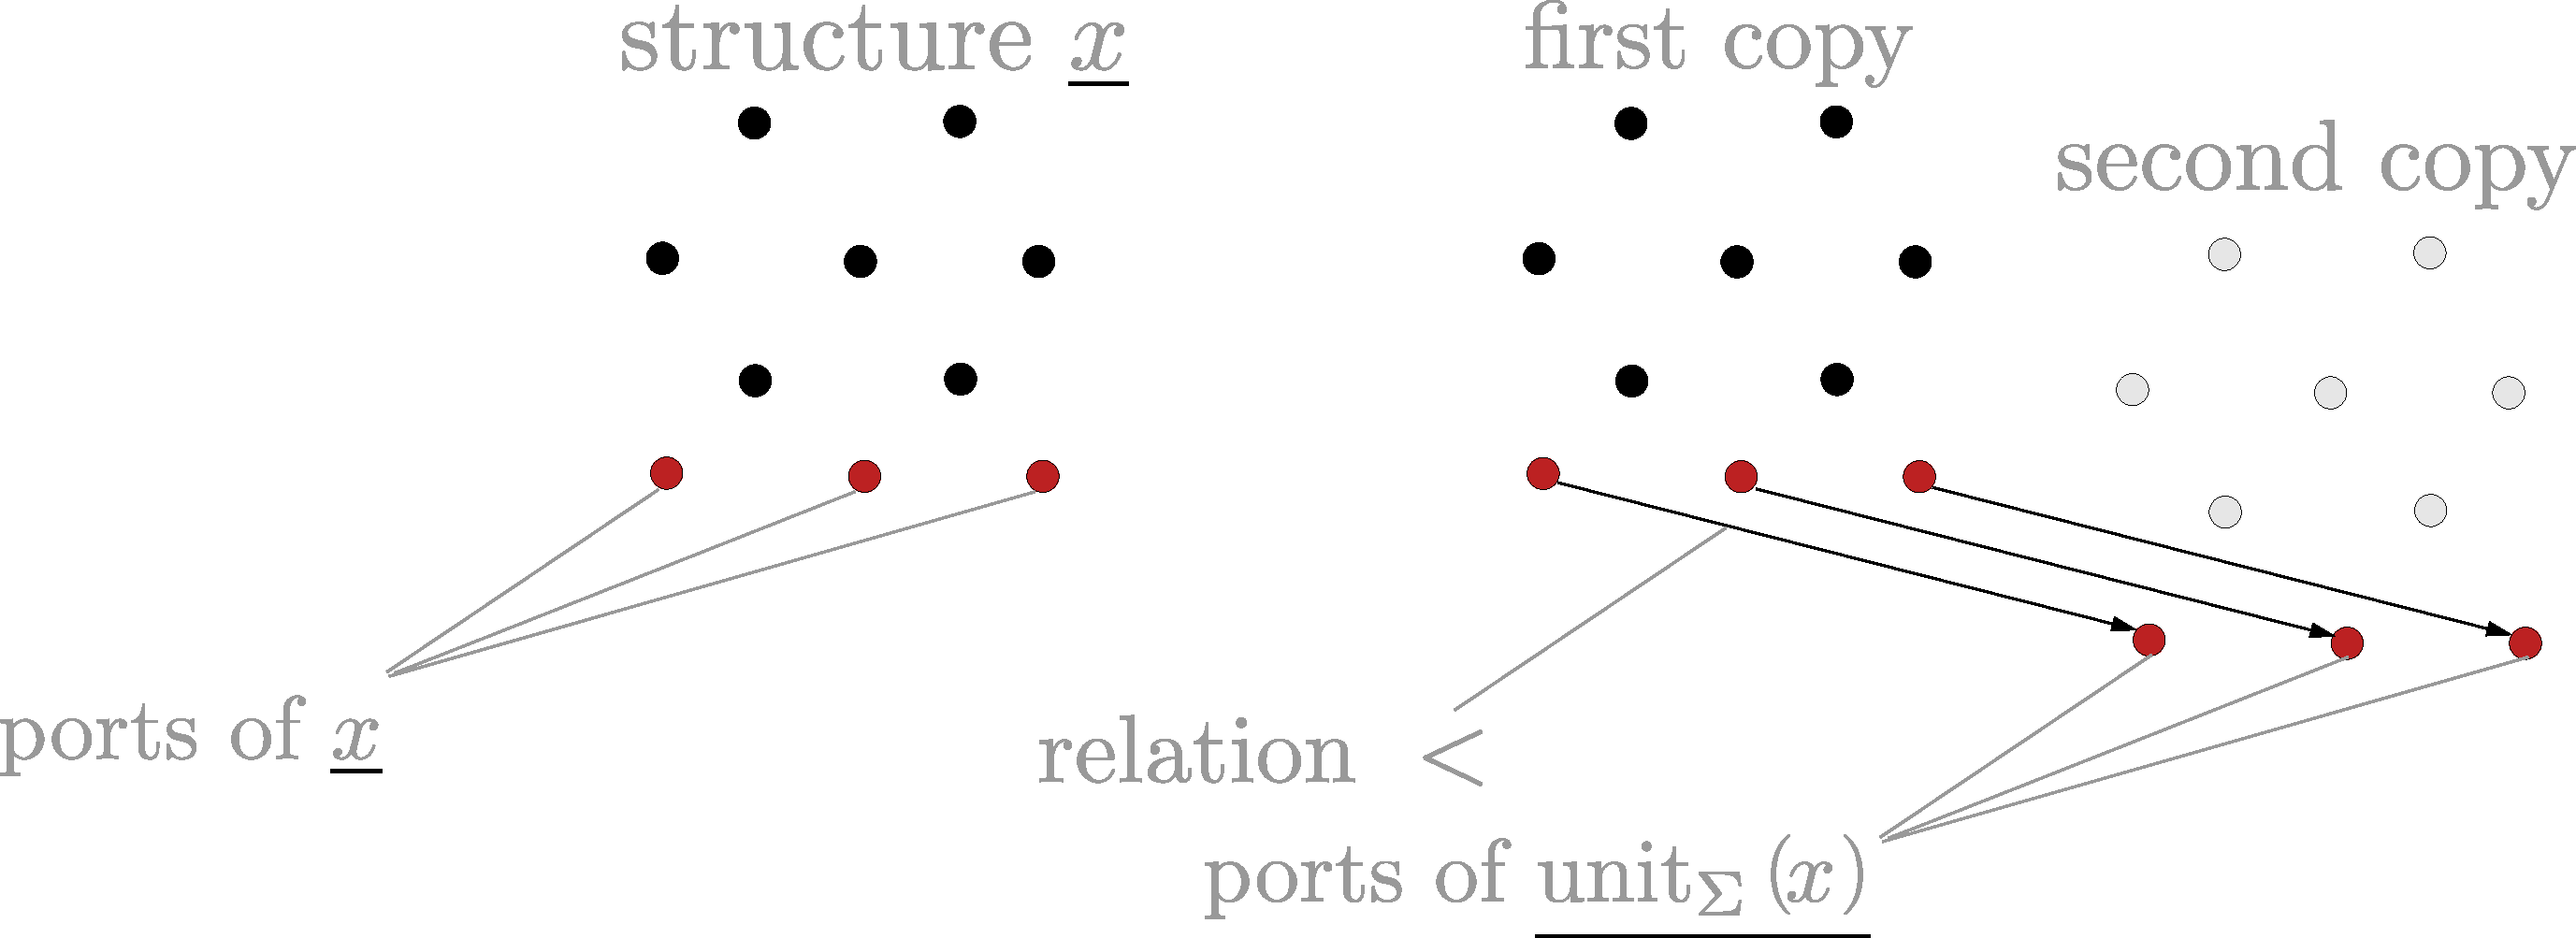
\includegraphics[scale=.18]{pictures/to-logic-unit.pdf}
    \end{center}    
      The universe formulas are then:
    \begin{align*}
    \varphi_1(x)=\mathsf{True} \qquad \varphi_2(x)=\mathsf{Port}_\rSigma(x)
    \end{align*}
    In the first copy, the vocabulary of $\rSigma$ will be interpreted as in the original structure, and as the empty set in the second copy. That is, for every unary relation $R$ and for every binary relation $S$ in the vocabulary of  $\rSigma$, we set:
    \begin{align*}
   \varphi_R^{1}(x)=R(x) \quad&\quad \varphi_S^{1,1}(x,y)=S(x,y)\\
   \varphi_R^{2}(x)=\mathsf{False} \quad&\quad \varphi_S^{2,2}(x,y)=\mathsf{False}
\end{align*}      
Let us interpret the relations $<$ and $\sqsubset$ of the vocabulary of $\tmonad\rSigma$. The  ports of $\underline{\unit(x)}$ inherit the order of the ports of $\underline{x}$, this is why we set:
\begin{align*}
\varphi_\sqsubset^{2,2}(x,y)=x\sqsubset_\rSigma y
\end{align*}
The descendant relation $<$ connects the $i^{th}$ port of $\underline{x}$ to the $i^{th}$ port of $\underline{\unit(x)}$. Since these nodes come from the same node in the original structure, we set:
\begin{align*}
\varphi_<^{1,2}(x,y)=x=y
\end{align*}